 % use the "wcp" class option for workshop and conference
 % proceedings
 %\documentclass[gray]{jmlr} % test grayscale version
 %\documentclass[tablecaption=bottom]{jmlr}% journal article
 \documentclass[tablecaption=bottom,wcp]{jmlr} % W&CP article

\usepackage{booktabs}
\usepackage{bm,amsmath,amssymb,algorithmic,algorithm}
\usepackage{graphicx}
\usepackage{xargs}


%%%%%%%%%%%%%%%%%%%%%%%%%%%%%%%%%%%%%%%%%%%%%%%%%%%%%%%%%%%
%%%%%    Comments shorcuts   			       %%%%%
%%%%%%%%%%%%%%%%%%%%%%%%%%%%%%%%%%%%%%%%%%%%%%%%%%%%%%%%%%%

%%%%%%%%%%%%%%%%%%%%%%%%%%%%%%%%%%%%%%%%%%%%%%%%%%%%%%%%%%%
%%%%%  		 latin abbreviations                  %%%%%
%%%%%%%%%%%%%%%%%%%%%%%%%%%%%%%%%%%%%%%%%%%%%%%%%%%%%%%%%%%
\newcommand{\ie}{{\em i.e.,~}}
\newcommand{\wlg}{{\em w.l.o.g.,~}}
\newcommand{\eg}{{\em e.g.,~}}
\newcommand{\lcf}{{\em cf.~}}
\newcommand{\resp}{{\em resp.~}}
\newcommand{\etal}{{\em et al.~}}
\newcommand{\wrt}{{\em w.r.t.~}}

%%%%%%%%%%%%%%%%%%%%%%%%%%%%%%%%%%%%%%%%%%%%%%%%%%%%%%%%%%%
%%%%%  		 Style mathbb                         %%%%%
%%%%%%%%%%%%%%%%%%%%%%%%%%%%%%%%%%%%%%%%%%%%%%%%%%%%%%%%%%%
\def\EE{\mathbb{E}}
\def\PP{\mathbb{P}}
\def\NN{\mathbb{N}}
\def\JJ{\mathbb{J}}
\def\E{\mathbf{E}}
\def\W{{\bf W}}
\def\X{{\bm X}}
\def\Z{{\bm Z}}
\def\StocEstep{{\bm{\mathcal{S}}}}
%\def\X{{\bm X}}
% \newcommand{\1}{\mathds{1}} %dsfont
\newcommand{\1}{\mathbbm{1}} %mathbbm

\newcommand{\beq}{\begin{equation}}
\newcommand{\eeq}{\end{equation}}
\newcommand{\beo}{\begin{array}{rl}}
\newcommand{\eeo}{\end{array}}
\newcommand{\ds}{\displaystyle}

%%%%%%%%%%%%%%%%%%%%%%%%%%%%%%%%%%%%%%%%%%%%%%%%%%%%%%%%%%%
%%%%%  		 Style mathcal                         %%%%%
%%%%%%%%%%%%%%%%%%%%%%%%%%%%%%%%%%%%%%%%%%%%%%%%%%%%%%%%%%%

\def\mcX{\mathcal{X}}
\def\mcY{\mathcal{Y}}

%%%%%%%%%%%%%%%%%%%%%%%%%%%%%%%%%%%%%%%%%%%%%%%%%%%%%%%%%%%
%%%%%  		 bullet symbols                       %%%%%
%%%%%%%%%%%%%%%%%%%%%%%%%%%%%%%%%%%%%%%%%%%%%%%%%%%%%%%%%%%

\def\startri{\star \star \star}
\def\stardble{\star\star\phantom{\star}}
\def\starone{ \star\!\!\!\phantom{\star\star\star}}
\def\iid{i.i.d.}
\def\eqs{\;}

%%%%%%%%%%%%%%%%%%%%%%%%%%%%%%%%%%%%%%%%%%%%%%%%%%%%%%%%%%%
%%%%%  		 defintion symbols                    %%%%%
%%%%%%%%%%%%%%%%%%%%%%%%%%%%%%%%%%%%%%%%%%%%%%%%%%%%%%%%%%%
\newcommand{\deq}{\stackrel{\Delta}{=}}

%%%%%%%%%%%%%%%%%%%%%%%%%%%%%%%%%%%%%%%%%%%%%%%%%%%%%%%%%%%
%%%%%  		 TODO and comments                    %%%%%
%%%%%%%%%%%%%%%%%%%%%%%%%%%%%%%%%%%%%%%%%%%%%%%%%%%%%%%%%%%
\usepackage{color}
\newcommand*{\TODO}[1]{\textbf{\textcolor{red}{TO~DO: #1}}}


%%%%%%%%%%%%%%%%%%%%%%%%%%%%%%%%%%%%%%%%%%%%%%%%%%%%%%%%%%%
%%%%%    Theorems etc. 			               %%%%%
%%%%%%%%%%%%%%%%%%%%%%%%%%%%%%%%%%%%%%%%%%%%%%%%%%%%%%%%%%%
%\theoremstyle{plain}
%\newtheorem{theorem}{Theorem}%[section]
%\newtheorem{definition}[theorem]{Definition}%[section]
%\newtheorem{lemma}[theorem]{Lemma}%[section]
%\newtheorem{proposition}[theorem]{Proposition}%[section]
%\newtheorem{corollary}[theorem]{Corollary}
%
%% \theoremstyle{remark}
%\newtheorem{remark}{Remark}%[section]
%%\theoremstyle{plain}
% \newtheorem{assumption}{H \hspace*{-5.5pt}}
%\newtheorem{problem}{P}
%\newcommand*{\assumptionrefname}{H}
% \newcommand*{\propositionrefname}{Proposition}
% \providecommand*{\assumptionautorefname}{H\!\!\!\!\!\!}  %hspace is stretchable, but \! is not and \!\! is too much
%\providecommand*{\problemautorefname}{(P)\hspace*{-3.5pt}}  %hspace is stretchable, but \! is not and \!\! is too much
%\providecommand*{\corollaryautorefname}{Corollary\hspace*{0pt}}

%%%%%%%%%%%%%%%%%%%%%%%%%%%%%%%%%%%%%%%%%%%%%%%%%%%%%%%%%%%
%%%%%    DeclarMathOperator 		               %%%%%
%%%%%%%%%%%%%%%%%%%%%%%%%%%%%%%%%%%%%%%%%%%%%%%%%%%%%%%%%%%

\DeclareMathOperator{\sign}{sign}
\DeclareMathOperator{\tr}{tr}
\DeclareMathOperator{\rank}{rk}
\DeclareMathOperator{\diag}{diag}
\DeclareMathOperator{\Proj}{\mathcal{P}}
\DeclareMathOperator{\Lik}{\Phi_Y}
\DeclareMathOperator{\Likpi}{\Phi_Y^\Pi}
\def\glik{\Sigma_Y}
\def\speq{-}

%%%%%%%%%%%%%%%%%%%%%%%%%%%%%%%%%%%%%%%%%%%%%%%%%%%%%%%%%%%
%%%%%    Functions 	 		               %%%%%
%%%%%%%%%%%%%%%%%%%%%%%%%%%%%%%%%%%%%%%%%%%%%%%%%%%%%%%%%%%

\newcommand{\argmin}{\mathop{\mathrm{arg\,min}}}
\newcommand{\Breg}[3]{d_{ #1 }(#2,#3)}
\newcommand{\HX}[2]{H_{#1} ( #2 )}
\newcommandx{\PX}[2][1=]{{P}^{#1}_{\prm_{#2}}}
\newcommandx{\PPX}[2]{{P}^{#1}_{\prm_{#2}}}
\newcommand{\hHX}[2]{\hat{H}_{{#1}} ( #2 )}

\newcommandx{\inter}[1][1={1,n}]{\llbracket #1\rrbracket}
\newcommandx{\Xset}[1][1=i]{\mathsf{X}_{#1}}
\newcommand{\prob}{\mathbb{P}}
\newcommand\infsum[1][n]{\ensuremath{\sum_{#1=-\infty}^\infty}}

\newcommand{\Bregemp}[2]{D^n_\Gexp(#1,#2)}
\newcommand{\Bregg}[2]{D(#1,#2)}
\newcommand{\Bregpi}[2]{D_\Gexp(#1,#2)}

\newcommand{\argmax}{\mathop{\mathrm{arg\,max}}}
\newcommand{\nul}[2]{ \mathrm{0}_{#1 \times #2} }

\newcommand{\scha}[1]{\| #1 \|_{\sigma,1}}
\newcommand{\mat}[1]{#1}
\newcommand{\ten}[1]{\mathcal{#1}}
\newcommand{\tenset}[3]{\RR^{#1 \times #2 \times #3 }}
\newcommand{\matset}[2]{\RR^{#1 \times #2}}
\newcommand{\mrk}[1]{\operatorname{\rank}(#1)}
\newcommand{\hs}[1]{\hat{\bm s}^{(#1)}}
\newcommand{\hp}[1]{\hat{\param}^{(#1)}}
\newcommand{\os}{\overline{\bm s}}
\newcommand{\op}{\overline{\param}}

\newcommand{\rth}{\bar{r}}
\newcommand{\Dn}{\operatorname{D}_{n,Y}}
\newcommand{\dhe}{d_H}
\newcommand{\Obj}{f}
\newcommand{\Objo}{\Phi}
\DeclareMathOperator{\Liko}{\Phi}
\DeclareMathOperator{\expo}{exp}
\DeclareMathOperator{\Ber}{Ber}
\newcommand{\Bern}[1]{#1}
\newcommand{\Lc}{\nu}
\newcommand{\const}{\kappa}
\newcommand{\Curve}{C_{\Obj}}
\newcommand{\Eob}{q}
\newcommand{\grd}{{\nabla}}
\newcommand{\Hgrd}{\hat{\nabla}}
\newcommand{\Tgrd}{\tilde{\nabla}}
\newcommand{\prm}{\bm{\eta}}
\newcommand{\Prm}{\mathcal{H}}
\newcommand{\Tprm}{\tilde{\bm{\theta}}}
\newcommand{\Bprm}{\overline{\bm{\theta}}}
\newcommand{\TPrm}{\tilde{\bm{\Theta}}}
\newcommand{\alp}{\bm{\alpha}}
\newcommand{\atom}{{\bm a}}
\newcommand{\lgp}{{ \rm A}}
\newcommand{\lgpm}{{ \mathcal{ A}}}
\newcommand{\bms}{{ \rm m}}
\newcommand{\Cset}{{\cal C}}
\newcommand{\scv}{\mu}
\newcommand{\Y}{{\bm Y}}
\newcommand{\exs}{T}
\newcommand{\noise}{\eta^\Delta}
\newcommand{\rtrust}{\overline{\bm W}}
\newcommand{\rB}{\overline{\bm B}}
\newcommand{\rD}{\overline{\bm D}}
\newcommand{\barx}{\overline{\bm x}}
\newcommand{\targetx}{{\bm x}^{target}}
\newcommand{\B}{{\bm B}}
\newcommand{\D}{{\bm D}}
\newcommand{\I}{{\bm I}}
\newcommand{\trust}{{\bm W}}
%%%%%%%%%%%%%%%%%%%%%%%%%%%%%%%%%%%%%%%%%%%%%%%%%%%%%%%%%%%
%%%%%    exponential law		               %%%%%
%%%%%%%%%%%%%%%%%%%%%%%%%%%%%%%%%%%%%%%%%%%%%%%%%%%%%%%%%%%
\newcommand{\sexp}{\lambda}
\newcommand{\Gexp}{G}
\newcommand{\gexp}{G'}
\newcommand{\dgexp}{G''}
\newcommand{\explaw}{Exp}
%%%%%%%%%%%%%%%%%%%%%%%%%%%%%%%%%%%%%%%%%%%%%%%%%%%%%%%%%%%
%%%%%    Missing from ERIC		               %%%%%
%%%%%%%%%%%%%%%%%%%%%%%%%%%%%%%%%%%%%%%%%%%%%%%%%%%%%%%%%%%
\newcommand{\eqdef}{\mathrel{\mathop:}=}
\newcommand{\pscal}[2]{\big\langle#1\,|\,#2 \big\rangle}
\newcommand{\Pscal}[2]{\Big\langle#1\,|\,#2\Big\rangle}
%%%%%%%%%%%%%%%%%%%%%%%%%%%%%%%%%%%%%%%%%%%%%%%%%%%%%%%%%%%
%%%%%    FOR EXPERIMENTS SECTION		       %%%%%
%%%%%%%%%%%%%%%%%%%%%%%%%%%%%%%%%%%%%%%%%%%%%%%%%%%%%%%%%%%
\def\iset{\ensuremath{\mathbb{K}}}
\def\Class{p}
\def\qClass{q}
\def\class{j}
\def\qclass{l}
\def\lmo{\rm top}
\def\ST{ {\rm ST}}
\def\stcv{K_\gamma}
\def\sigup{\bar{\sigma}}
\def\siglo{\underline{\sigma}}
\def\mtop{\bar{M}}
\def\mlo{\underline{M}}
\def\tens{\mathcal{M}}
\def\schat_const{s}
\def\wrec{W}
\def\lip{L}
\def\Xmin{X^*}
\def\cbern{c^*}
\newcommand{\supp}{\operatornamewithlimits{supp}}
\DeclareMathOperator{\Lin}{\mathcal{Q}}
% \usepackage[ruled,vlined]{algorithm2e}
\newcommand{\Objb}{\tilde{\Phi}_Y^{\lambda}}
\newcommand{\Objob}{\tilde{\Phi}_{\lambda}}
\def\rset{\ensuremath{\mathbb{R}}}
\newcommand{\eqsp}{\;}
\newcommand{\empf}[2]{ \Delta^2_Y (#1, #2) }
\newcommand{\empfw}[2]  { \sum _{kl \in [m_1] \times [m_2]} \pi_{kl} (#1_{kl} - #2_{kl})^2 }
\newcommand{\KL}[2]{\operatorname{KL}\left(#1,#2\right)}
\newcommand{\KLd}[2]{{D}\left(#1\|#2\right)}
\newcommand{\rscset}[2]{ \mathcal{C}(#1,#2) }
\newcommand{\rscsett}[3]{ \mathcal{C}(#1,#2,#3) }
\newcommand{\dhel}[2]{\operatorname{d_h}\left(#1,#2\right)}
\newcommand{\dhes}[2]{\operatorname{d_H^2}\left(#1,#2\right)}
\newcommand{\jacob}[3]{\operatorname{J}_{#1}^{#2}(#3)}
\newcommand{\hess}[2]{\operatorname{H}_{#1}^{#2}}
\newcommand{\mstep}[1]{\overline{\param}({#1})}
\def\PE{\mathbb{E}}
\def\prox{prox}
\def\tX{\bar{\prm}}
\def\tT{\bar{T}}
\def\est{\hat{\mat{X}}}
\def\gradpi{H}
\def\estpi{\check{\mat{X}}}
\def\bvarepsilon{\boldsymbol{\varepsilon}}
\def\bE{\mathbf{E}}
\newcommand{\Exp}[3]{\operatorname{Exp}_{#1,#2,#3}}
\def\bY{\mathbf{Y}}
\def\indic{\delta}
\def\contset{\mathcal{C}}
\def\contsetr{\mathcal{A}}
\def\rme{\mathrm{e}}
\newcommand{\norm}[1]{\left\Vert #1 \right\Vert}
\newcommand{\normop}[1]{\| #1 \|_{\sigma,\infty}}
\newcommand{\normfr}[1]{\| #1 \|_{\sigma,2}}
\newcommand{\normtr}[1]{\| #1 \|_{\sigma,1}}
\def\mrc{K}
%\newcommand{\mrc}[1]{K(#1)}
\def\link{l}
\def\lu{{\rm U}}
\def\lv{ {\rm V} }
\def\lcoef{{\rm \theta }}
\def\AA{{\cal A} }
%\crefname{table}{Table}{Tables}
%\Crefname{algocf}{Algorithm}{Algorithms}
% \crefname{proposition}{Proposition}{Propositions}
% % \providecommand*{\porpositionrefname}{Proposition}

%% \newcommand*{\propositionrefname}{Proposition}
%% \newcommand*{\propositionsrefname}{Propositions}
%% \newcommand*{\propositionref}[1]{%
%%   \objectref{#1}{\propositionrefname}{\propositionsrefname}{}{}}

%%% definitions of sets
\def\rset{\ensuremath{\mathbb{R}}}
\def\rsetbar{\ensuremath{\bar{\rset}}}
\def\rplus{\ensuremath{\rset_+}}
\def\qset{\ensuremath{\mathbb{Q}}}
\def\nset{\ensuremath{\mathbb{N}}}
\def\zset{\ensuremath{\mathbb{Z}}}
\def\cset{\ensuremath{\mathbb{C}}}
\def\Xset{\mathsf{X}}
\def\Yset{\mathsf{Y}}
\def\Zset{\mathsf{Z}}
\def\Xsigma{\mathcal{X}}
\def\param{{\bm{\theta}}}
\def\Param{\Theta}
\def\Rker{R}
\def\borelA{\mathsf{A}}
\def\borelSet{\mathcal{B}}
\def\borel{\mathcal{B}}
\newcommand{\coint}[1]{\left[#1\right)}
\newcommand{\ocint}[1]{\left(#1\right]}
\newcommand{\ooint}[1]{\left(#1\right)}
\newcommand{\ccint}[1]{\left[#1\right]}
\def\invpi{\pi}
\def\pibar{\bar{\pi}}
\newcommand{\toi}[1]{\todo[color=green!20]{{\bf TO:} #1}}
\newcommand{\eric}[1]{\todo[color=red!20]{{\bf EM:} #1}}
\newcommand{\erici}[1]{\todo[color=red!20,inline]{{\bf EM:} #1}}
\newcommand{\belhal}[1]{\todo[color=green!20]{{\bf BK:} #1}}
\newcommand{\belhali}[1]{\todo[color=green!20,inline]{{\bf BK:} #1}}


\newcommand{\toco}[1]{\todo[color=yellow!20]{{\bf To:} #1}}
\def\rmd{\mathrm d}
\def\mcf{\mathcal{F}}
\def\be{\bm{e}}
\def\State{X}
\def\state{x}
\def\TV{\operatorname{TV}}


\newcommandx{\indi}[2][1=]{\1^{#1}_{#2}}
\newcommand{\indiacc}[1]{\1_{\{#1\}}}
\newcommand{\indin}[1]{\1\left\{#1\right\}}

\newcommandx{\CPE}[3][1=]{{\mathbb E}_{#1}\left[\left. #2 \, \right| #3 \right]} %%%% esperance conditionnelle
\newcommandx{\CPP}[3][1=]
{\ifthenelse{\equal{#1}{}}{{\mathbb P}\left(\left. #2 \, \right| #3 \right)}{{\mathbb P}_{#1}\left(\left. #2 \, \right | #3 \right)}}

\def\Sset{\mathsf{S}}
\def\Aset{\mathsf{A}}
\def\Reward{\operatorname{R}}
\def\transMDP{\operatorname{P}}
\def\Policy{\Pi}
\def\invarMDP{\upsilon}
\def\Pen{\operatorname{R}}
\def\calL{{\mathcal{L}}}
\def\bss{{\mathbf{s}}}

\def\iter{\delta}

\def\bssdoc{\overline{{\mathbf{s}}}^{(t|d)}}
\def\bsstop{\overline{{\mathbf{s}}}^{(w|t)}}

\def\surrogate{Q}
\newcommand{\Lip}[1]{\operatorname{L}_{#1}}
\newcommand{\ensemble}[2]{\left\{#1\,:\eqsp #2\right\}}
\newcommand{\set}[2]{\ensemble{#1}{#2}}
\def\calS{\mathcal{S}}
\def\Cat{\operatorname{Cat}}
\def\Dir{\operatorname{Dir}}
\def\pardocpost{{\bm{\vartheta}}^{(\mathrm{d})}}
\def\partoppost{{\bm{\vartheta}}^{(\mathrm{t})}}
\def\pardoc{\param^{(\mathrm{t|d})}}
\def\partop{\param^{(\mathrm{w|t})}}
\def\opardoc{\overline{\param}^{(\mathrm{t|d})}}
\def\opartop{\overline{\param}^{(\mathrm{w|t})}}



\newcommand{\estpardoc}[1]{\big( \param_{d,k}^{(\mathrm{t|d})} \big)^{#1}}
\newcommand{\estpartop}[1]{\big(\param_{k,v}^{(\mathrm{w|t})} \big)^{#1}}

\newcommand{\probasimplex}[1]{\mathcal{P}_{#1}}
\def\obsdoc{y^{(\mathrm{d})}}
\def\obsword{y^{(\mathrm{w})}}
\def\bomega{\boldsymbol{\omega}}
\def\bmu{\boldsymbol{\mu}}

\def\ISAEM{iSAEM}
\def\SAEMVR{vrSAEM}
\def\FISAEM{fiSAEM}

\jmlrproceedings{AABI 2020}{3rd Symposium on Advances in Approximate Bayesian Inference, 2020}

 % The optional argument of \title is used in the header
\title[Hyperparameters Weight Averaging in BNNs]{HWA: Hyperparameters Weight Averaging in Bayesian Neural Networks}


% Anonymous authors (leave as is; do not reveal author names for your submission)
\author{\Name{Anonymous Authors}\\
  \addr Anonymous Institution}
% THE SUBMISSION MUST REMAIN ANONYMOUS

% Two authors with the same address
% \author{\Name{Author Name1\nametag{\thanks{A note}}} \Email{abc@sample.com}\and
%  \Name{Author Name2} \Email{xyz@sample.com}\\
%  \addr Address}


\begin{document}

\maketitle


\begin{abstract}
Bayesian neural networks attempt to combine the strong predictive performance of neural networks with formal quantification of uncertainty associated with the predicted output in the Bayesian framework
%Bayesian Deep Learning presents itself as the most useful tool for adding uncertainty estimation to traditional Deep Learning models that only produce point estimates predictions as outputs. 
Confidence of the model and the predictions at inference time are left alone. Applying randomness and Bayes Rule to the weights of a deep neural network is a step towards achieving this goal. Current state of the art optimization methods for training Bayesian Neural Networks are relatively slow and inefficient, compared to their deterministic counterparts. In this paper, we propose \textsc{HWA} (Hyperparameters Weight Averaging) algorithm that leverages an averaging procedure in order to train faster and achieve better accuracy. We develop our main algorithm using the simple averaging heuristic and demonstrate its effectiveness on the space of the hyperparameters of the neural networks random weights. Numerical applications are presented to confirm the empirical benefits of our method.
\end{abstract}

\section{Introduction}
While Deep Learning methods have shown increasing efficiency in various domains such as natural language processing, computer vision or robotics, sensible areas including autonomous driving or medical imaging not only require accurate predictions but also uncertainty quantification.
In~\citep{neal2012bayesian}, authors develop a bayesian variant of plain feedforward multilayer neural networks in which weights and biases are considered as random variables.
For supervised learning tasks, deterministic models are prone to overfitting and are not capable of estimating uncertainty in the training data resulting in making overly confident decisions about the correct class, \textit{i.e.} miscalibration~\citep{guo2017calibration,kendall2017uncertainties}.
Nevertheless, representing that aforementioned uncertainty is crucial for decision making.
Bayesian methods display a hierarchical probabilistic model that assume a (prior) random distribution over the parameters of the parameters and are useful for assessing the uncertainty of the model via posterior predictive distribution quantification~\citep{blundell2015weight,kingma2015variational}.
Current training methods for Bayesian Neural Networks (BNN)~\citep{neal2012bayesian} include Variational Inference~\citep{graves2011practical, hoffman2013stochastic} or BayesByBackprop~\citep{blundell2015weight} based on Evidence Lower Bound (ELBO) maximization task.
Naturally, Bayesian methods, and in particular BNNs, are thus highly sensitive to the parameters choice of the prior distribution and current state-of-the-art models are not as efficient and robust as traditional deep learning models.

In this paper, we introduce a new \emph{optimization} algorithm to alleviate those challenges.
Our main contributions read as follows:
\begin{itemize}
\item We introduce Hyperparameter Weight Averaging (HWA), a training algorithm that leverages stochastic averaging techniques~\citep{polyak1992acceleration} and posterior sampling methods.
\item Given the high nonconvexity of the loss landscape, our method finds heuristic explanation from theoretical works on averaging and generalization such as~\citep{keskar2016large,he2019asymmetric} and more practical work on Deep Neural Networks (DNN) optimization such as~\citep{izmailov2018averaging}.

\item We provide numerical examples showcasing the effectiveness of our method on simple and complex supervised classification tasks.
\end{itemize}

The remaining of the paper is organized as follows.
Section~\ref{sec:related} presents the related works in the fields of optimization, Variational Inference and posterior sampling.
Section~\ref{sec:main} introduces our main contribution, namely the HWA algorithm.
Section~\ref{sec:numerical} highlights the benefits of our procedure on various classification tasks.
Section~\ref{sec:conclusion} concludes our work.

%\textbf{Notations:} We denote for all $n >1$, $[n]$ the set $ \{1, \cdots, n\}$, $\pi(w)$ denotes the prior distribution on the vector of random weights $w$.
 
\section{Related Work}\label{sec:related}

\textbf{Posterior Prediction.}
Due to the nonconvexity of the loss landscapes involved in modern and complex deep learning tasks, direct sampling from the posterior distribution of the weights is not an option.
Depending on the nature and in particular the dimensionality of the problem, Markov Chain Monte Carlo (MCMC) methods have been employed to overcome this intractability issue.
By constructing a Markov chain, the samples drawn at convergence are guaranteed to be drawn from the target distribution.
Hamiltonian Monte Carlo (HMC)~\citep{neal2011mcmc} or Metropolis Hastings (MH)~\citep{hastings1970monte} are two standard solutions used.
Their stochastic gradients counterpart are extensively studied in \citep{ma2015complete}.

\vspace{0.08in}
\noindent \textbf{Variational Inference (VI).}
When tackling an optimization problem, exact posterior sampling may be computationally involved and not even required.
variational inference was proposed in~\citep{graves2011practical}, in the particular case of BNNs, in order to fit a Gaussian variational posterior approximation over the weights of neural networks.
Through a simple reparameterization trick~\citep{blundell2015weight}, several methods have emerged to train BNNs leveraging the ease of use and implementation of VI~\citep{kingma2015variational,blundell2015weight,molchanov2017variational}.
Though, those methods appear to be inefficient for large-scale datasets and newer methods were proposed to alleviate this issue such as the use of normalizing flows~\citep{louizos2017multiplicative}, deterministic VI~\citep{wu2018deterministic} or dropout VI~\citep{gal2016dropout}.

\vspace{0.08in}
\noindent \textbf{Stochastic Averaging.}
Averaging methods include the seminal papers of~\citep{polyak1990sa} and~\citep{ruppert1988efficient}, both based on the combination of past iterates along a stochastic approximation trajectory.
For nonconvex objectives, this averaging procedure has been adapted to Stochastic Gradient Descent (SGD) trajectory in \citep{zhou2017convergence}.
In particular, in modern deep learning examples, \citet{izmailov2018averaging} develops a novel method that averages snapshots of a DNN through the iterations and shows better empirical generalization.
Those experimental discoveries are then backed by theoretical understanding of the loss landscape in~\citep{keskar2016large,he2019asymmetric}.


\section{Hyperparameters Averaging in Bayesian Neural Networks}\label{sec:main}

In this section, we introduce the basic concepts of Bayesian Neural Networks and their corresponding loss function which plays a key role in this paper.
From an optimization perspective, we review the Stochastic Weight Averaging (SWA)~\citep{izmailov2018averaging} averaging procedure, which can be seen as an approximation of the mean trajectory of the SGD iterates and introduce our method, namely HWA.
\textit{While SWA averages snapshots of the weights of the neural networks from past and successive iterations, our method HWA only captures snapshots of the hyperparameters, and not of the weights that are sampled at each training iteration.}
We then discuss the uncertainty estimation prediction of such method and how our proposed extra step combining \emph{posterior sampling} and \emph{optimization} can lead to a better generalization of the trained model on test sets.

\subsection{Bayesian Neural Networks and ELBO Maximization}
Let $((x_i,y_i),  i \in [n])$ be i.i.d.~input-output pairs and $w \in \mathcal{W} \subseteq \mathbb{R}^{d}$ be a latent variable. When conditioned on the input data $x = (x_i, i \in [n])$, the joint distribution of $y = (y_i, i \in [n])$ and $w$ is given by:
\begin{equation}\label{eq:vi} \textstyle
    p(y,w | x) = \prior(w)\prod_{i=1}^{n}{p(y_i | x_i, w)} \eqsp.
\end{equation}

In the particular case of BNN, this likelihood function is parametrized by a multilayer neural network, which can be convolutional or not.
The latent variables $w$ are thus the weights and the biases of the model and are considered as latent (and random) variables.
Training of such hierarchical models implies sampling from the posterior distribution of the weights $w$ conditioned on the data $(x,y)$ and noted $p(w|y,x)$.
In most cases, this posterior distribution $p(w|y,x)$ is intractable and is approximated using a family of parametric distributions, $\{q(w, \param ), \param \in \Param \}$. 
The variational inference (VI) problem~\citep{blei2017variational} boils down to minimizing the Kullback-Leibler (KL) divergence between $q(w, \param )$ and the posterior distribution $p(w|y,x)$. The tractable objective is the ELBO (Evidence Lower BOund) written as:
\begin{equation}\label{eq:variationalobjective}
{\cal L}(\param) \eqdef -\EE_{ q( w; \param )} \big[\log p(y | x, w) \big]+  \EE_{ q( w; \param )} \big[ \log q(w; \param )/\prior(w) \big]  \eqsp.
\end{equation}
%\begin{equation} \label{eq:VI}  
%\min_{ \param \in \Param }~{\cal L}(\param ) \eqdef \infdiv{q(w; \param )}{p(w|y,x)} \eqdef \EE_{ q( w; \param )} \big[ \log \big( q(w; \param ) / p(w|y,x) \big) \big] \eqsp,
%\end{equation}
Directly optimizing the objective function in \eqref{eq:variationalobjective} can be difficult.
First, with $n \gg 1$, evaluating the objective function ${\cal L}( \param )$ requires a full pass over the entire dataset.
Second, for some complex models, the expectations in \eqref{eq:variationalobjective} can be intractable even if we assume a simple parametric model for $q(w; \param)$.
Thus, the computation of the gradient requires an approximation step usually invoking Monte Carlo (MC) approximation step. 
The full Variational inference procedure for training Bayesian Neural Networks, including \textit{the MC approximation} step and the \textit{parameter update} step, is summarized in Algorithm~\ref{alg:trainingbnn}.

Solutions simply include using SGD~\citep{bottou2008tradeoffs} where the gradient of the individual ELBO~\eqref{eq:variationalobjective} is computed using Automatic Differentiation~\citep{kucukelbir2017automatic}. 
The final update goes in the opposite direction of that gradient up to a learning rate factor.
In the sequel, we develop an improvement over baseline SGD, invoking averaging virtue of several successive snapshots of the gradients.
The method, called Hyperparameters Weight Averaging (HWA), aims at improving the generalization property of the trained model on unseen data.


\subsection{Averaging model snapshots through hyperparameters loss landscapes}
Consider a deterministic deep neural network, the idea behind the Stochastic Weight Averaging (SWA) procedure, developed in~\citep{izmailov2018averaging} , is to run several iterates of the classical SGD procedure, starting from a pre-trained model.
At each timestep noted $T_{\mathsf{avg}}$, the model estimate is equal to the average of the last $T_{\mathsf{avg}}$ iterates.
%Empirically, a constant and large learning rate is more efficient given the exploration virtue that it implies.
After establishing the connectivity between several modes (point estimate of minimal loss) of the same deep neural network (after different training procedure) in~\citep{garipov2018loss}, being able to average all those iterates probably traversing several models or at least model estimates that belong to low loss region would make the resulting trained model more robust and thus generalize better to unseen data.
Several theoretical paper such as~\citep{he2019asymmetric} or \citep{keskar2016large} provide an attempt at explaining this phenomena.


\textbf{-- Hyperparameters Weight Averaging:}
Based on the probabilistic model developed above, the loss function~\eqref{eq:variationalobjective} is defined on the space of the hyperparameters, \textit{i.e.} the mean and the variance of the variational candidate distribution.
Regarding the parameterization choice of the variational candidate $q( w; \param )$, we chose for simplicity a scalar mean $\mu_{\ell}$ depending on the layer $\ell \in [L]$ and constant between each neuron. Classically, the covariance of this variational distribution is diagonal, see~\citep{kirkpatrick2017overcoming, blundell2015weight}, yet can be too restrictive.
We follow the direction taken in~\citep{maddox2019simple}, where the covariance of $q(w, \param)$ is a diagonal matrix.
As a result, the averaging procedure practically occurs on the set of hyperparameters and requires updating the mean and the variance of the variational candidate distribution, at iteration $k+1$, if $k$, the iteration index, is a multiple of the cycle length $c$,  as below:
\begin{equation}\label{eq:hwa_updates}
\begin{split}
 \mu_{\ell}^{HWA}  =  \frac{n_{\textrm{m}}\mu_{\ell}^{HWA} + \mu_{\ell}^{k+1}}{n_{\textrm{m}}+1}  \quad \textrm{and} \quad  \sigma^{HWA}   =  \frac{n_{\textrm{m}}\sigma^{HWA} + (\mu_{\ell}^{k+1})^2}{n_{\textrm{m}}+1} -( \mu_{\ell}^{HWA})^2 \, ,
\end{split}
\end{equation}
where for all $\ell \in [L]$, $\mu_{\ell}^{k+1}$ and $\sigma^{k+1}$ are both obtained via Stochastic Variational Inference.


\begin{algorithm}[H]
\algsetup{indent=0.25em}
\begin{algorithmic}[1]
\STATE \textbf{Input:} Iteration index $k$. Trained hyperparameters $\hat{\mu}_{\ell}$ and $\hat{\sigma}$. LR $\gamma_k$. Cycle length $c$. Gradient vector $\nabla \mathcal{L}_{i_{k}}(\theta^{k})$
%\STATE Initialize the hyperparameters of the weights and 
%$\mu_{\ell} = \hat{\mu}_{\ell}$ and $\mu^{HWA}_{\ell} = \mu_{\ell}$.
\STATE $\gamma \leftarrow \gamma(k)$ (Cyclical LR for the iteration)
\STATE \textbf{SVI updates:}
\STATE \quad $\mu_{\ell}^{k+1} \leftarrow \mu_{\ell}^{k} - \gamma_k \nabla_{\mu_{\ell}} \mathcal{L}_{i_{k}}(\mu_{\ell}^{k})$  \label{line:svi}
\STATE \quad $\sigma^{k+1} \leftarrow \sigma^{k} - \gamma_k \nabla_{\sigma} \mathcal{L}_{i_{k}}(\sigma^{k})$ \label{line:svisigma}
\IF{$\textrm{mod}(k,c) = 0$}
	\STATE \quad $n_{\textrm{m}} \leftarrow k/c$ \quad (Number of models to average over)
\begin{equation}\notag
\mu_{\ell}^{HWA} \leftarrow \frac{n_{\textrm{m}}\mu_{\ell}^{HWA} + \mu_{\ell}^{k+1}}{n_{\textrm{m}}+1} \quad \textrm{and} \quad \sigma^{HWA} \leftarrow \frac{n_{\textrm{m}}\sigma^{HWA} + (\mu_{\ell}^{k+1})^2}{n_{\textrm{m}}+1} -( \mu_{\ell}^{HWA})^2
\end{equation}
\ENDIF
\STATE \textbf{Return} hyperparameters $(\{\mu_{\ell}^{HWA}\}_{l=1}^L, \sigma^{HWA})$.
\end{algorithmic}
\caption{HWA: Hyperparameters Weight Averaging}
\label{alg:hwa}
\end{algorithm}

Algorithm~\ref{alg:hwa} develops the main method of our paper.
Stochastic Variational update is executed Line~\ref{line:svi}.
The stochastic averaging procedure happens every $c$ iterations, and consists in computing the weight sum between the latest model estimate and the running average noted using the superscript $\textrm{HWA}$.

Note that in the above procedure, the variational candidate $q(w, \param)$ has a diagonal covariance matrix where the scalar standard deviations are obtained through Algorithm~\ref{alg:hwa}.
One parameter estimates are updated via \eqref{eq:hwa_updates}, the neural network weights are then sampled according to the updated variational candidate distributions in order to compute the next iteration approximate stochastic gradient $\nabla \mathcal{L}_{i_{k}}(\theta)$.
Yet it is also possible build a non diagonal proposal covariance to bypass the restriction of such structure.
Besides, given the nonconvexity and high dimensionality of the true posterior distribution, adding even a low rank non diagonal structure to the covariance of our proposal would yield a gain in efficiency in the variational inference procedure.
Of course the ideal option would be to build a posterior curvature-informed covariance but at a higher cost.
The trade-off between computational costs and proposal efficiency is detailed in the following.
The low-rank plus diagonal posterior approximation matrix, noted $\Sigma$ of $q(w, \param)$ introduced in \citep{maddox2019simple} reads:
\begin{equation}\label{eq:lowrankcov}
\Sigma = \frac{1}{2} \Sigma_{\text {diag }}+\frac{\widehat{D} \widehat{D}^{\top}}{2(R-1)}
\end{equation}
where $\mu^{HWA} = (\mu_{\ell}^{HWA}, \ell \in [L])$, $R$ is the maximum number of columns in the low rank deviation matrix $\widehat{D}$ and $\Sigma_{\text {diag }}$ is the diagonal covariance defined above. The $r$-th component, where $r \in [R]$, of the  low rank deviation matrix $\widehat{D}$ is defined as the gap between the current estimate and the running average: $\widehat{D}_r = \theta_r - \theta^{HWA}_r$. It quantifies how far the current estimate parameter deviate from the current averaged parameter.

Then the covariance of the proposal $q(\cdot)$ in Algorithm~\ref{alg:trainingbnn} is either set to \eqref{eq:hwa_updates} or \eqref{eq:lowrankcov}

Several hyperparameters are worth highlighting here.
The standard learning rate $\gamma_k$ plays a key role and is either equal to a constant or a cyclical learning rate.
The cycle length $c$ which monitors the number of times snapshots of the model estimates are being averaged is also of utmost importance and needs careful tuning.

%
%\subsection{Variational Inference with HWA}
%Note that in the above procedure, the variational candidate $q(w, \param)$ has a diagonal covariance matrix where the scalar standard deviations are obtained through Algorithm~\ref{alg:hwa}.
%One parameter estimates are updated via \eqref{eq:hwa_updates}, the neural network weights are then sampled according to the updated variational candidate distributions in order to compute the next iteration approximate stochastic gradient $\nabla \mathcal{L}_{i_{k}}(\theta)$.
%Yet it is also possible build a non diagonal proposal covariance to bypass the restriction of such structure.
%Besides, given the nonconvexity and high dimensionality of the true posterior distribution, adding even a low rank non diagonal structure to the covariance of our proposal would yield a gain in efficiency in the variational inference procedure.
%Of course the ideal option would be to build a posterior curvature-informed covariance but at a higher cost.
%The trade-off between computational costs and proposal efficiency is detailed in the following.
%The low-rank plus diagonal posterior approximation matrix, noted $\Sigma$ of $q(w, \param)$ introduced in \citep{maddox2019simple} reads:
%\begin{equation}\label{eq:lowrankcov}
%\Sigma = \frac{1}{2} \Sigma_{\text {diag }}+\frac{\widehat{D} \widehat{D}^{\top}}{2(R-1)}
%\end{equation}
%where $\mu^{HWA} = (\mu_{\ell}^{HWA}, \ell \in [L])$, $R$ is the maximum number of columns in the low rank deviation matrix $\widehat{D}$ and $\Sigma_{\text {diag }}$ is the diagonal covariance defined above. The $r$-th component, where $r \in [R]$, of the  low rank deviation matrix $\widehat{D}$ is defined as the gap between the current estimate and the running average: $\widehat{D}_r = \theta_r - \theta^{HWA}_r$. It quantifies how far the current estimate parameter deviate from the current averaged parameter.
%
%Then the covariance of the proposal $q(\cdot)$ in Algorithm~\ref{alg:trainingbnn} is either set to \eqref{eq:hwa_updates} or \eqref{eq:lowrankcov}.
%
%\textbf{Discussion on the choice of the variational candidate distribution:} 
%The general aim of the update rules presented above is to construct an efficient variational candidate distribution that would provide an approximate shape of the true posterior. Our method acts on the mean and covariance of a simple Gaussian distribution where the covariance matrix is either diagonal or low rank.
%Nevertheless, other choice of proposal can be employed such as the spike and slab variational distribution, in \citep{gal2016dropout}, leveraging dropout mechanism in VI. 
%The other similar idea, namely concrete dropout in \citep{gal2017concrete} not only optimizes the hyperparameters of the weights but also the dropout probabilities.
%We do not consider those variants as our work focuses on Gaussian approximations of the posterior distribution and how their parameters are updated, see Section~\ref{sec:numerical} for a description of baseline methods used in our numerical experiments.
%
%
%We now give in Algorithm~\ref{alg:trainingbnn}, the overall training algorithm of the Bayesian Neural Network using the proposed HWA algorithm to update the parameters.
%\begin{algorithm}[H]
%\algsetup{indent=0.25em}
%\begin{algorithmic}[1]
%\STATE \textbf{Input:} Trained hyperparameters $\hat{\mu}_{\ell}$ and $\hat{\sigma}$. Sequence of LR $\{\gamma_k\}_{k > 0}$. Cycle length $c$. $K$ iterations.
%\FOR {$k=0,1,...$}
%\STATE Sample an index $i_k$ uniformly on $[n]$
%\STATE Sample MC batch of weights $\{w^m_k\}_{m=1}^{M_k}$  from variational candidate $q(w, \theta^k)$ with $\theta^k = (\mu^k, \Sigma^k)$ and the covariance is either diagonal~\eqref{eq:hwa_updates} or low rank~\eqref{eq:lowrankcov}.
%\STATE Compute MC approximation of the gradient vectors:
%$$ \nabla \mathcal{L}_{i_{k}}(\theta^{k}) \approx \frac{1}{M_k} \sum_{m=1}^{M_k} \log p(y_{i_k} | x_{i_k}, w^k_m)  + \nabla KL(q(w, \theta^k)||\pi(w)) $$
%\STATE Update the vector of parameter estimates calling Algorithm~\ref{alg:hwa}: $(\mu^K, \Sigma^K) =  \textsc{HWA}(k, c, \gamma_k, \nabla \mathcal{L}_{i_{k}}(\theta^{k}) )$
%\ENDFOR
%\STATE \textbf{Return} Fitted parameters $(\mu^K, \Sigma^K)$.
%\end{algorithmic}
%\caption{Variational Inference with HWA for BNNs}
%\label{alg:trainingbnn}
%\end{algorithm}



\section{Numerical Experiments}\label{sec:numerical}
We provide experiments on classification tasks with various neural network architectures and datasets to demonstrate the effectiveness of method, namely HWA.

\noindent \textbf{Methods.}\hspace{0.1in}
We consider two baselines: standard \textsc{BayesByBackprop} method developed in~\citep{blundell2015weight} and the Stochastic Gradient Langevin Dynamics (SGLD) optimization method introduced in~\citep{welling2011bayesian}.
The algorithms are initialized at the same point and the results are averaged over 5 repetitions.


\noindent \textbf{Datasets.}\hspace{0.1in}
We compare different algorithms on \textit{MNIST}~\citep{lecun-mnisthandwrittendigit-2010} and \textit{CIFAR10}~\citep{krizhevsky2009learning} datasets.
%The \textit{MNIST} training set is composed of $n=55\,000$ handwritten digits, $28 \times 28$ images. Each image is labelled with its corresponding number (from zero to nine).
%\textit{CIFAR10} is a popular computer-vision datasets of $50\,000$ training images and $10\,000$ test images, of size $32\times 32$. 

\noindent \textbf{Network architectures.} \hspace{0.1in}
(MNIST) We train a Bayesian variant of LeNet-5 convolutional neural network on the MNIST dataset. 
Under the prior distribution $\prior$, see \eqref{eq:vi}, the weights are assumed  independent and identically distributed according to ${\cal N}(0,1)$.
We also assume a Gaussian variational candidate distribution such that $q(\cdot; \param) \equiv  \mathcal{N}(\mu,\sigma^2 \Id )$.
The variational posterior parameters are thus $\param = (\mu, \sigma) $ where $\mu = (\mu_\ell, \ell \in [d])$ where $d$ is the number of weights in the neural network. 
(CIFAR-10) We train here the Bayesian variant of the VGG neural network introduced in~\citep{simonyan2014very} on the CIFAR-10 dataset.
As in the previous example, the weights are assumed i.i.d. according to ${\cal N}(0,\Id)$.
Standard hyperparameters values found in the literature, such as the annealing constant or the number of MC samples, were used for the benchmark methods. 
For better efficiency and lower variance, the Flipout estimator~\citep{wen2018flipout} is used.

\noindent \textbf{Results.} \hspace{0.1in} 
Results for both datasets and network architectures are reported Figure~\ref{fig:all}.
While for the MNIST dataset the runs for \textsc{HWA} and \textsc{SGLD} are com:parage both in terms of train and testing loss and accuracy, they both highlights better convergence properties compared to \textsc{BayesByBackprop} (BBB).
It is worth mentioning that our method \textsc{HWA} displays a similar behavior as a gradient based method, such as \textsc{SGLD}, by only leveraging the average of past snapshots of the variational candidate hyperparameters. 
Regarding the CIFAR10 experiment, our method shows overfitting on training data with respect to the loss objective but seems to generalize better to unseen data (cf. last figure on bottom line in Figure~\ref{fig:all}).
In conclusion, \textsc{HWA} achieves state-of-the-art results for either small or large bayesian variants of standard network architectures while using a simple and efficient averaging update at each \textit{cycle}.



\begin{figure}[H]
\mbox{
\includegraphics[width=0.25\textwidth]{newfigs/MNIST_train_loss.eps}
\includegraphics[width=0.25\textwidth]{newfigs/MNIST_train_acc.eps}
\includegraphics[width=0.25\textwidth]{newfigs/MNIST_test_loss.eps}
\includegraphics[width=0.25\textwidth]{newfigs/MNIST_test_acc.eps}
}
\mbox{
\includegraphics[width=0.25\textwidth]{newfigs/CIFAR_train_loss.eps}
\includegraphics[width=0.25\textwidth]{newfigs/CIFAR_train_acc.eps}
\includegraphics[width=0.25\textwidth]{newfigs/CIFAR_test_loss.eps}
\includegraphics[width=0.25\textwidth]{newfigs/CIFAR_test_acc.eps}
}
 \caption{Comparison for Bayesian LeNet CNN architecture on MNIST dataset (top) and Bayesian VGG architecture on CIFAR-10 dataset (bottom). The plots are averaged over 5 repetitions.}
\label{fig:all}
\end{figure}


\section{Conclusion}\label{sec:conclusion}
We present in this paper an averaging procedure on the hyperparameters of the weights of a Bayesian Neural Network architecture.
Based on both empirical and theoretical results regarding stochastic averaging, we propose HWA in order to increase the generalization ability of a BNN.
The procedure is easily implementable on top of any vanilla optimizer with standard design choices for prior and candidate distributions, crucial in variational inference.
Numerical runs show the advantage of our method matching and sometimes beating SOTA methods such as SGLD, which requires additional expensive gradient computation.

%\acks{Acknowledgements go here.}

\clearpage

\bibliography{ref}

\clearpage
\appendix

  \hsize\textwidth
  \linewidth\hsize \toptitlebar {\centering
  {\Large\bfseries Appendix for HWA: Hyperparameters Weight Averaging in Bayesian Neural Networks \par}}
 \bottomtitlebar 
 
\section{Comparison with other classical averaging procedures in nonconvex optimization}
From Algorithm~\ref{alg:hwa}, we note that the averaging procedure happens once at each cycle $c$, a tuning hyperparameter, on the parameter estimates resulting from a simple stochastic gradient descent update.
Yet, another natural averaging step would be to keep $K$ snapshots of the past stochastic gradients and compute an aggregated sum used as the drift term in the general update rule, see \citep{zhou2017convergence}.
Nevertheless, in our setting, the objective function while being nonconvex is (possibly) parameterized by a high dimensional neural network making it computationally involved to store those $K$ gradients.


\textbf{Incremental Aggregated Gradients methods:} Popular optimization methods, such as SAG~\citep{schmidt2017minimizing} or SAGA~\citep{defazio2014saga}, make use of the past individual gradient and compute a moving average of those vectors as the final drift term. Those methods are proven to be faster than plain SGD in both convex and nonconvex cases, leveraging among other reasons variance reduction effect, but suffer from a high storage cost. Indeed the drift term is composed of the sum of the $n$ past individual gradient where $n$ is equal to the size of the training set.


\textbf{MISO~\citep{mairal2015incremental}:} Another important method invoking variance reduction through incremental update of the drift term in a gradient descent step is the Minimization by Incremental Surrogate Optimization method, namely MISO, developed in \citet{mairal2015incremental}.
Contrary to the method mentionned above, the accumulation does not happen on the gradient but on the sum of individual surrogate objective functions.
While this framework is more general than SAG or SAGA, and also does not require storing $n$ past gradients, it is still computationally heavy to store those $n$ past objective functions, rather their model parameter estimates, when tackling deep neural networks training.

For all those reasons, \textsc{HWA} surely combines the virtue of the accumulation/aggregation effect and the low computing cost of vanilla SGD.



\section{Embedding HWA in Variational Inference}
Note that in the above procedure, the variational candidate $q(w, \param)$ has a diagonal covariance matrix where the scalar standard deviations are obtained through Algorithm~\ref{alg:hwa}.
One parameter estimates are updated via \eqref{eq:hwa_updates}, the neural network weights are then sampled according to the updated variational candidate distributions in order to compute the next iteration approximate stochastic gradient $\nabla \mathcal{L}_{i_{k}}(\theta)$.
Yet it is also possible build a non diagonal proposal covariance to bypass the restriction of such structure.
Besides, given the nonconvexity and high dimensionality of the true posterior distribution, adding even a low rank non diagonal structure to the covariance of our proposal would yield a gain in efficiency in the variational inference procedure.
Of course the ideal option would be to build a posterior curvature-informed covariance but at a higher cost.
The trade-off between computational costs and proposal efficiency is detailed in the following.
The low-rank plus diagonal posterior approximation matrix, noted $\Sigma$ of $q(w, \param)$ introduced in \citep{maddox2019simple} reads:
\begin{equation}
\Sigma = \frac{1}{2} \Sigma_{\text {diag }}+\frac{\widehat{D} \widehat{D}^{\top}}{2(R-1)}
\end{equation}
where $\mu^{HWA} = (\mu_{\ell}^{HWA}, \ell \in [L])$, $R$ is the maximum number of columns in the low rank deviation matrix $\widehat{D}$ and $\Sigma_{\text {diag }}$ is the diagonal covariance defined above. The $r$-th component, where $r \in [R]$, of the  low rank deviation matrix $\widehat{D}$ is defined as the gap between the current estimate and the running average: $\widehat{D}_r = \theta_r - \theta^{HWA}_r$. It quantifies how far the current estimate parameter deviate from the current averaged parameter.

Then the covariance of the proposal $q(\cdot)$ in Algorithm~\ref{alg:trainingbnn} is either set to \eqref{eq:hwa_updates} or \eqref{eq:lowrankcov}.

\textbf{Discussion on the choice of the variational candidate distribution:} 
The general aim of the update rules presented above is to construct an efficient variational candidate distribution that would provide an approximate shape of the true posterior. Our method acts on the mean and covariance of a simple Gaussian distribution where the covariance matrix is either diagonal or low rank.
Nevertheless, other choice of proposal can be employed such as the spike and slab variational distribution, in \citep{gal2016dropout}, leveraging dropout mechanism in VI. 
The other similar idea, namely concrete dropout in \citep{gal2017concrete} not only optimizes the hyperparameters of the weights but also the dropout probabilities.
We do not consider those variants as our work focuses on Gaussian approximations of the posterior distribution and how their parameters are updated, see Section~\ref{sec:numerical} for a description of baseline methods used in our numerical experiments.


We now give in Algorithm~\ref{alg:trainingbnn}, the overall training algorithm of the Bayesian Neural Network using the proposed HWA algorithm to update the parameters.
\begin{algorithm}[H]
\algsetup{indent=0.25em}
\begin{algorithmic}[1]
\STATE \textbf{Input:} Trained hyperparameters $\hat{\mu}_{\ell}$ and $\hat{\sigma}$. Sequence of LR $\{\gamma_k\}_{k > 0}$. Cycle length $c$. $K$ iterations.
\FOR {$k=0,1,...$}
\STATE Sample an index $i_k$ uniformly on $[n]$
\STATE Sample MC batch of weights $\{w^m_k\}_{m=1}^{M_k}$  from variational candidate $q(w, \theta^k)$ with $\theta^k = (\mu^k, \Sigma^k)$ and the covariance is either diagonal~\eqref{eq:hwa_updates} or low rank~\eqref{eq:lowrankcov}.
\STATE Compute MC approximation of the gradient vectors:
$$ \nabla \mathcal{L}_{i_{k}}(\theta^{k}) \approx \frac{1}{M_k} \sum_{m=1}^{M_k} \log p(y_{i_k} | x_{i_k}, w^k_m)  + \nabla KL(q(w, \theta^k)||\pi(w)) $$
\STATE Update the vector of parameter estimates calling Algorithm~\ref{alg:hwa}: $(\mu^K, \Sigma^K) =  \textsc{HWA}(k, c, \gamma_k, \nabla \mathcal{L}_{i_{k}}(\theta^{k}) )$
\ENDFOR
\STATE \textbf{Return} Fitted parameters $(\mu^K, \Sigma^K)$.
\end{algorithmic}
\caption{Variational Inference with HWA for BNNs}
\label{alg:trainingbnn}
\end{algorithm}

\end{document}
